% Created 2016-04-22 Fri 03:05
\documentclass[12pt,twoside]{article}
\usepackage[utf8]{inputenc}
\usepackage[T1]{fontenc}
\usepackage{fixltx2e}
\usepackage{graphicx}
\usepackage{longtable}
\usepackage{float}
\usepackage{wrapfig}
\usepackage{rotating}
\usepackage[normalem]{ulem}
\usepackage{amsmath}
\usepackage{textcomp}
\usepackage{marvosym}
\usepackage{wasysym}
\usepackage{amssymb}
\usepackage{hyperref}
\tolerance=1000
\usepackage{tabularx}
\usepackage{minted}
\usepackage[paper=a4paper,dvips,top=1.5cm,left=1.5cm,right=1.5cm, foot=1cm,bottom=1.5cm]{geometry}
\renewcommand{\rmdefault}{ptm}
\usepackage[scaled=.90]{helvet}
\usepackage{courier}
\usepackage{bookmark}
\usepackage{fancyhdr}
\pagestyle{fancy}
\usepackage[dvipsnames*,svgnames]{xcolor}
\usepackage{tikz}
\usetikzlibrary{arrows,decorations.pathmorphing,backgrounds,fit,positioning,calc,shapes}
\usepackage[utf8]{inputenc}
\usepackage[swedish, english]{babel}
\usepackage{rotating}
\usepackage{array}
\usepackage{graphicx}
\usepackage{float}
\usepackage{color}
\usepackage{mdwlist}
\usepackage{setspace}
\usepackage{listings}
\usepackage{bytefield}
\usepackage{tabularx}
\usepackage{multirow}
\usepackage{algorithm}
\usepackage{algpseudocode}
\usepackage{dcolumn}
\usepackage{url}
\usepackage[perpage,para,symbol]{footmisc}
\usepackage[all]{hypcap}
\definecolor{darkblue}{rgb}{0.0,0.0,0.3} %% define a color called darkblue
\definecolor{darkred}{rgb}{0.4,0.0,0.0}
\definecolor{red}{rgb}{0.7,0.0,0.0}
\definecolor{lightgrey}{rgb}{0.8,0.8,0.8}
\definecolor{grey}{rgb}{0.6,0.6,0.6}
\definecolor{darkgrey}{rgb}{0.4,0.4,0.4}
\hyphenpenalty=15000
\tolerance=1000
\newcommand{\rr}{\raggedright}
\newcommand{\rl}{\raggedleft}
\newcommand{\tn}{\tabularnewline}
\newcommand{\colorbitbox}[3]{%
\rlap{\bitbox{#2}{\color{#1}\rule{\width}{\height}}}\bitbox{#2}{#3}}
\newcommand{\red}{\color{red}}
\makeatletter
\renewcommand\paragraph{\@startsection{paragraph}{4}{\z@}{-3.25ex\@plus -1ex \@minus -.2ex}{1.5ex \@plus .2ex} {\normalfont\normalsize\bfseries}}
\makeatother
\makeatletter
\renewcommand\subparagraph{\@startsection{subparagraph}{5}{\z@}{-3.25ex\@plus -1ex \@minus -.2ex}{1.5ex \@plus .2ex} {\normalfont\normalsize\bfseries}}
\makeatother
\setcounter{tocdepth}{3}
\setcounter{secnumdepth}{5}
\renewcommand{\headrulewidth}{0pt}
\lhead{Konstantinos Sotiropoulos}
\chead{Ms Thesis Intermediate Report}
\rhead{\date{\today}}
\makeatletter
\let\ps@plain\ps@fancy
\makeatother
\setlength{\headheight}{15pt}
\author{Konstantinos Sotiropoulos \\ \texttt{kisp@kth.se}}
\date{\today}
\title{Parallel Simulation of SystemC Loosely-Timed Transaction Level Models}
\hypersetup{
  pdfkeywords={},
  pdfsubject={},
  pdfcreator={Emacs 24.5.1 (Org mode 8.2.10)}}
\begin{document}

\maketitle
\clearpage



\begin{abstract}
The vision of a connected and automated society, the Internet of Things era has promised,
is depending on the industry's ability to design novel and complex electronic systems,
while maintaining a short time to market.
One of the first steps in the design of such systems is the in tandem simulation of hardware and software.
Transaction Level Models, expressed in the SystemC modeling language, can facilitate this co-simulation.
However, the sequential nature of the SystemC's Discrete Event simulation kernel is a limiting factor.
Poor simulation performance often constraints the scope and depth of the design decisions that can be evaluated.

The increase in computing power, modern processing units deliver, is only avalailable for applications that can expose parallel operations.
The major obstacle one faces, when trying to parallelize a simulation, is the preservation of causality; simulation events need to be processed in a chronological order.

It is the main objective of this thesis' project to demonstrate the feasibility of parallelizing the simulation of Transaction Level Models, outside SystemC's reference simulation environment.
The difficult task of achieving causal, yet parallel, processing of simulation events, is accomplished by using proper process synchronization mechanisms.
Our proposed implementation does not depend on the presence of a centralized simulation moderator. 
It is implemented using the Message Passing Interface 3.0 framework.
To demonstrate our approach and evaluate different process synchronization algorithms,
we use the model of a cache-coherent, symmetric multiprocessor based on the OpenRisc 1000 Instruction Set Simulator. Our results indicate a significant speedup against the reference SystemC simulation.

Keywords: parallel discrete event simulation, conservative synchronization algorithms, transaction level models, SystemC TLM 2.0
\end{abstract}
\clearpage




\tableofcontents
\clearpage

\section*{Preface}
\label{sec-2}
This is a Master's Thesis project that will be carried out in Intel Sweden AB and is supervised by KTH's ICT department.
Mr. Bjorn Runaker (\texttt{bjorn.runaker@intel.com}) is the project's supervisor from the company's side, 
while professor \href{https://people.kth.se/~ingo/}{Ingo Sander} (\texttt{ingo@kth.se}) and PhD student \href{http://people.kth.se/~ugeorge/}{George Ungureanu} (\texttt{ugeorge@kth.se}) are the examiner and supervisor from KTH. 
The project begun on 2016-01-16 and will finish on 2016-06-30, as dictated by the contract of employment that I, Konstantinos Sotiropoulos a Master's student at the Embedded Systems program, have signed with the company.

The scope of this project has been mutually agreed on and dialectically determined between the company's needs and the institute's research agenda.
As Master's Thesis project, it will expose a scientific ground on which the engineering effort shall be rooted.

All the necessary equipment (software and hardware) has been kindly provided by the company.
The exact legal context that will apply to any software produced as a result of this project is yet to be determined, 
but will conform to the general context dictated by the documents already signed (documents' titles:  "Statement of Terms and Conditions of Fixed Term Employment" and "Employee Agreement") .
\clearpage


\section*{Acronyms}
\label{sec-1}
\begin{center}
\begin{tabular}{ll}
\textbf{ASIC}: & Application Specific Integrated Circuit\\
\textbf{DE}: & Discrete Event\\
\textbf{DES}: & Discrete Event Simulator/Simulation\\
\textbf{DMI}: & Direct Memory Interface\\
\textbf{ES}: & Electronic System\\
\textbf{ESLD}: & Electronic System-Level Design\\
\textbf{FPGA}: & Field Programmable Gate Array\\
\textbf{HDL} & Hardware Description Language\\
\textbf{HPC}: & High Performance Computing\\
\textbf{IC} & Integrated Circuit\\
\textbf{MoC}: & Model of Computation\\
\textbf{MPI} & Message Passing Interface\\
\textbf{MPSoC}: & Multicore System on Chips\\
\textbf{OoO}: & Out-of-Order\\
\textbf{PDES}: & Parallel Discrete Event Simulation\\
\textbf{SLDL}: & System-Level Design Language\\
\textbf{SMP}: & Symmetric Multiprocessing\\
\textbf{SoC}: & System on Chip\\
\textbf{SR}: & Synchronous Reactive\\
\textbf{TLM}: & Transaction Level Modeling\\
\textbf{CMB}: & Chandy/Misra/Bryant algorithm\\
\end{tabular}
\end{center}
\clearpage







\section{Introduction}
\label{sec-3}
The aim of this chapter is to present the general context of the problem statement.
that is the engineering discipline of \textbf{Electronic System-Level Design (ESLD)}.

In unit \ref{sec-3-1} we provide a definition for the fundamental concepts of design, system, model and simulation.
In units \ref{sec-3-2} to \ref{sec-3-4}, using Gajski and Kuhn's Y-Chart, we determine the concept of a Transaction-Level Model, as an instance in the engineering practice of Electronic System-Level Design (ESLD).
In unit \ref{sec-3-5} we have a rudimentary look on SystemC's role in ESLD.
The structure of this document is given in unit \ref{sec-3-6}.

\subsection{The Design Process}
\label{sec-3-1}
We define the process of \textbf{designing} as the engineering art of incarnating a desired functionality into a perceivable, thus concrete, artifact.
An engineering artifact is predominantly referred to as a \textbf{system}, 
to emphasize the fact that it can be viewed as a structured collection of components and that its behavior is a product of the interaction among its components.

Conceptually, designing implies a movement from abstract to concrete, fueled by the engineer's \textbf{design decisions}, incrementally adding implementation details.
This movement is also known as the \textbf{design flow} and can be facilitated by the creation of an arbitrary number of intermediate artifacts called models.
A \textbf{model} is thus an abstract representation of the final artifact. 
The design flow can be now semi-formally defined as a process of model refinement, with the ultimate model being the final artifact itself.
We use the term semi-formal to describe the process of model refinement, because to the best of our knowledge, 
such model semantics and algebras that would establish formal transformation rules and equivalence relations are far from complete \cite{Gajski2009}.

A desired property of a model is executability that is its ability to demonstrate portions of the final artifact's desired functionality in a controlled environment.
An \textbf{executable model}, allows the engineer to form hypotheses, conduct experiments on the model and finally evaluate design decisions.
It is now evident that executable models can firmly associate the design process with the scientific method.
The execution of a model is also known as \textbf{simulation} \cite{Editor2014}.


\subsection{Electronic Systems Design}
\label{sec-3-2}
An Electronic System (ES) provides a desired functionality, by manipulating the flow of electrons.
Electronic systems are omnipotent in every aspect of human activity; 
most devices are either electronic systems or have an embedded electronic system for their cybernisis.

The prominent way for visualizing the ES design/abstraction space is by means of the Y-Chart.
The concept was first presented in 1983 \cite{Gajski1983} and has been constantly evolving to capture and steer industry practices.
Figure \ref{fig:Y-Chart} presents the form of the Y-Chart found in \cite{Gajski2009}.

\begin{figure}[htb]
\centering
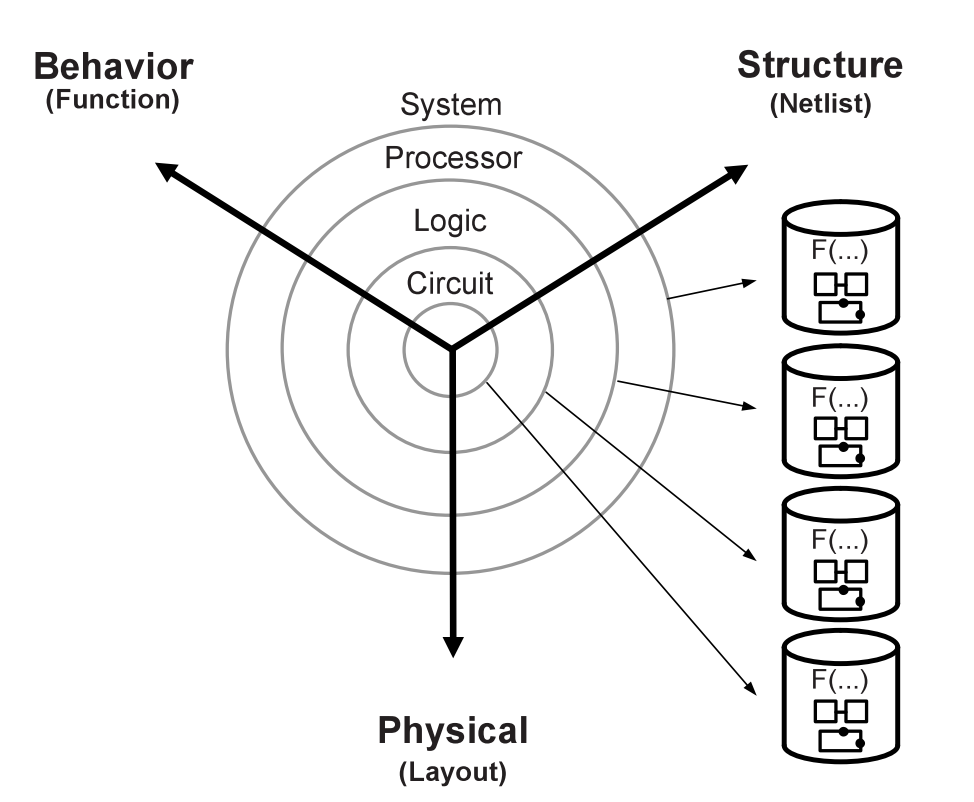
\includegraphics[scale=.45]{Figures/y-chart.png}
\caption{\label{fig:Y-Chart}The Y-Chart (adopted from \cite{Gajski2009})}
\end{figure}


The Y-Chart quantizes the design space into four levels of abstraction; system, processor, logic and circuit, represented as the four concentric circles.
For each abstraction level, one can use different ways for describing the system; behavioral, structural and physical.
These are represented as the three axises, hence the name Y-Chart.
Models can now be identified as points in this design space.

A typical design flow for an Integrated Circuit (IC) begins with a high-level behavioral model capturing the system's specifications and 
proceeds non-monotonically to a lower level structural representation, expressed as a netlist of, still abstract, components.
From there, Electronic Design Automation (EDA) tools will pick up the the task of reducing the abstraction of a structural model by translating the netlist of abstract components to a netlist of standard cells.
The nature of the standard cells is determined by the IC's fabrication technology (FPGA, gate-array or standard-cell ASIC).
Physical dimensionality is added by place and route algorithms, 
part of an EDA framework, 
signifying the exit from the design space, 
represented in the Y-Chart by the transition from the structural to the physical axis.

We have used the adjective non-monotonic to describe the design flow, because as a movement in the abstraction space, it is iterative; 
design $\rightarrow$ test/verify $\rightarrow$ redesign or proceed.
This cyclic nature of the design flow is implied by the errors the human factor introduces, under the lack of formal model transformation methodologies in the upper abstraction levels.
The term \textbf{synthesis} is therefore introduced to describe a monotonic movement from a behavioral to a structural model, or the realization of an upper level structural model using finer components.
We distinguish synthesis from the general case of the design flow, to disregard the testing and verification procedures.
Therefore, the term synthesis may indicate the presence, or the desire of having, an automated design flow.
Low-level synthesis is a reality modern EDA tools achieve, while high-level synthesis is still a utopia modern tools are converging to.


\subsection{System-Level Design}
\label{sec-3-3}
To meet the increasing demand for functionality, ES complexity, as expressed by their heterogeneity and their size, is increasing.
Terms like Systems on Chip (SoC) and Multi Processor SoC (MPSoC), used for characterizing modern ES, indicate this trend.
With abstraction being the key mental ability for managing complexity, the initiation of the design flow has been pushed to higher abstraction levels.
In the Y-Chart the most abstract level, depicted as the outer circle, is the system level.
At this level the distinction between hardware and software is a mere design choice thus \textbf{co-simulation of hardware and software} is one of the main objectives.
Thereby the term \textbf{system-level design} is used to describe design flows that enter the design space at this level.

A common practice among modern system-level design tools/methodologies, 
like Intel's CoFluent Studio \cite{citation}, 
is for the designer to construct two intermediate models;
An application model, that is the behavioral view of the system and 
a platform model, assembled using a component database of Processing Elements (PE, processors, hardware accelerators etc) and Communication Elements (CE, buses, interfaces etc).
The final step towards \textbf{system-level synthesis}, that is the transition from a behavioral to a structural model on the system level, is called system mapping;
the partitioning of the application to the elements of the platform.


\subsection{Transaction-Level Model}
\label{sec-3-4}
A \textbf{Transaction-Level Model} (TLM) can now be defined as the point in the Y-Chart where the structural axis meets the system abstraction level.
As mentioned in the previous unit, a TLM can be thought of as a platform model, or \textbf{virtual platform}, where an application can/is mapped \cite{Rigo2011}.
It is the model that facilitates co-simulation of hardware and software.
The notion of the transaction as an abstraction of communication will be clarified in chapter \ref{sec-6}.

What are the pragmatic reasons that make the development of a virtual platform imperative?
To begin with, an increasing amount of an ES's functionality is becoming software based. 
Moreover, ES related companies are facing the economical pressure of reducing new products' time to market.
Thus, software engineers must be equipped with a virtual platform they can use for software development, early on in the design flow, without needing to wait for the actual silicon to arrive.


\subsection{SystemC and TLM}
\label{sec-3-5}
One fundamental question, for completing the presentation of ESLD, remains; How can executable models be expressed on the system level?
While maintaining the expressiveness of a Hardware Description Language (HDL), \textbf{SystemC} is meant to act as an \textbf{Electronic System Level Design Language} (ESLDL);
a language with which system-level models can be expressed.
It is implemented as a C++ class library, thus its main concern is to provide the designer with executable rather than EDA synthesizable models.
The language is maintained and promoted by Accellera (former Open SystemC Initiative OSCI) and has been standardized (IEEE 1666-2011 \cite{OpenSystemCInitiative2012}).

\uline{COMMENT:} Why is SystemC regarded as Specific Domain Language (SDL)?
In what way does SystemC provide support for Transaction Level Modeling? Through the TLM 1.0 and 2.0 API.











\subsection{Document Overview}
\label{sec-3-6}
This unit be completed in the end
\clearpage



\section{Formulating The Problem Statement}
\label{sec-4}
The aim of this chapter is to present a theoretical framework that will eventually lead to the formulation of the problem statement.
Picking up Ariadne's thread from the introduction, this chapter begins its journey by the fact that SystemC is an Electronic System-Level Design \textbf{Language} (ESLDL) for expressing system-level models.

In unit \ref{sec-4-1} we link the concepts of operational semantics and Models of Computation (MoC) with that of the ESLDL.
In units \ref{sec-4-2} and \ref{sec-4-3} the SystemC simulation engine or kernel is presented as an algorithm that realizes the operational semantics of a Discrete Event (DE) MoC.
Units \ref{sec-4-4} and \ref{sec-4-5} introduce the concept of Parallel Discrete Event Simulation (PDES) and present the fundamental causality hazards it introduces.
The prime concern of this thesis' is presented in a concise way in \ref{sec-4-6}.
Unit \ref{sec-4-7} introduces the objectives, that is the engineering endeavor of this project.

\subsection{Models of Computation}
\label{sec-4-1}
A \textbf{language} is a set of symbols, rules for combining them (its syntax), and rules for interpreting combinations of symbols (its semantics). 
Two approaches to semantics have evolved: denotational and operational.
\textbf{Operational semantics}, which dates back to Turing machines, gives the meaning of a language in terms of actions taken by some abstract machine. 
How the abstract machine in an operational semantics can behave is a feature of what we call the \textbf{Model of Computation (MoC)} \cite{Edwards1997}.
This definition implies that languages are not computational models themselves, but have underlying computational models \cite{Jantsch2005}.

How does the concept of a MoC fit specifically in ESLDLs?
Above all the engineer needs executable models.
Furthermore, an ESLDL describes an electronic artifact as a system; a (hierarchical) network of interacting components.
Therefore, a MoC is a collection of rules to define what constitutes a component and what are the semantics of execution, communication and concurrency of the abstract machine that will execute the model \cite{Jantsch2005} \cite{Editor2014}.
To ensure meaningful simulations, the MoC of the abstract machine that simulates a model must be equivalent with that of the abstract machine that will realize the system.

\begin{figure}[htb]
\centering
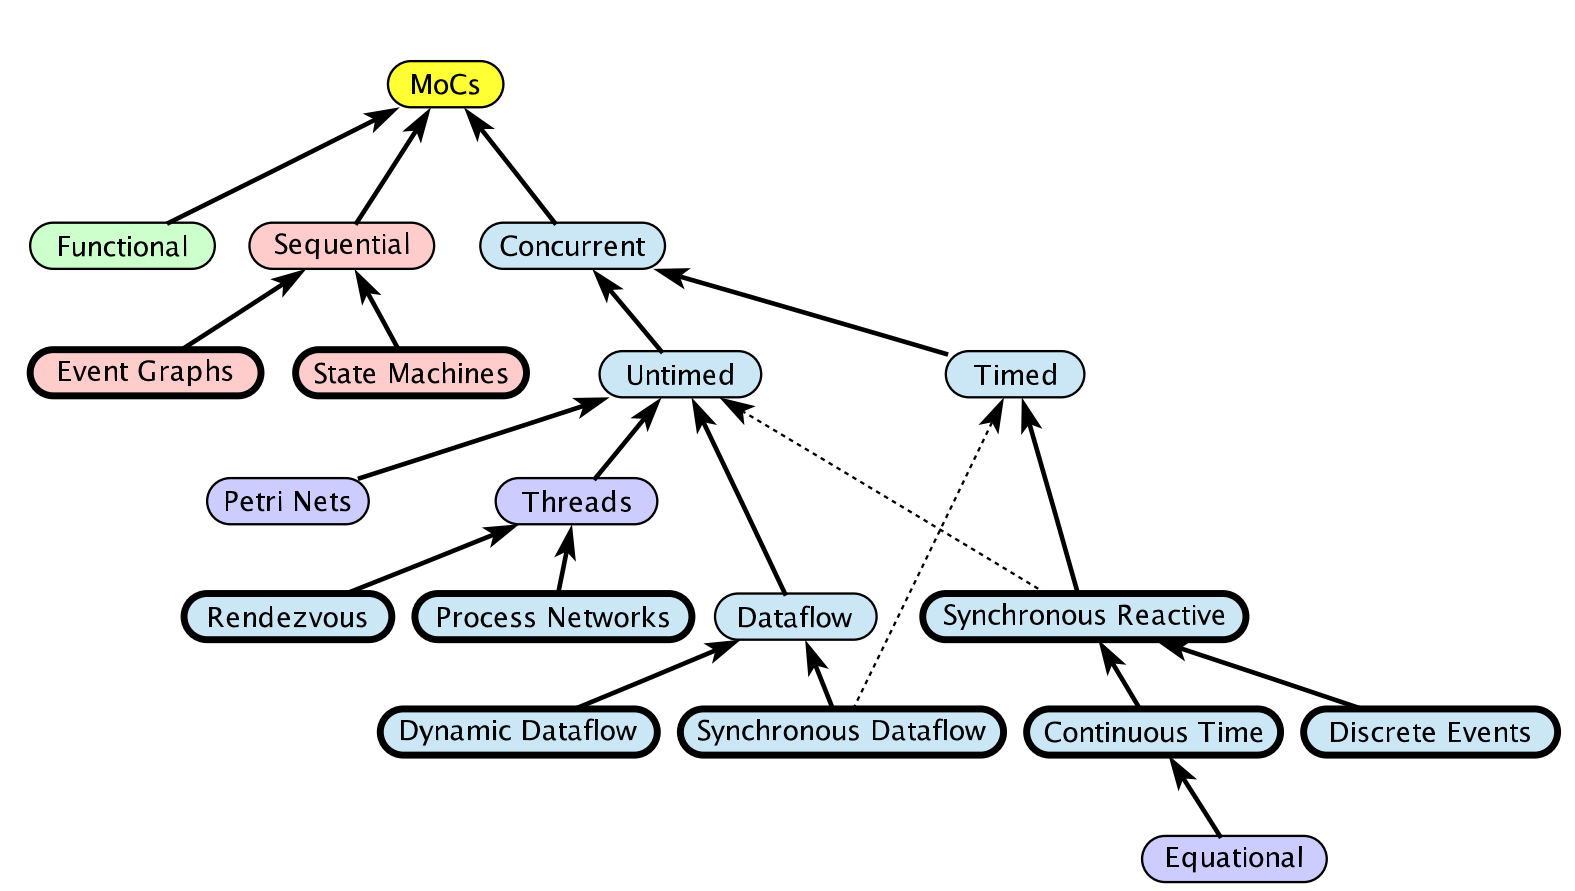
\includegraphics[scale=.45]{Figures/MoCs.png}
\caption{\label{fig:MoCs}Categorization of three of the most explored MoCs: State Machine, Synchronous Dataflow and Discrete Event(adopted from \cite{Editor2014})}
\end{figure}


\subsection{Discrete Event Model of Computation}
\label{sec-4-2}
The dominant MoC that underlies most industry standard HDLs (VHDL, Verilog, SystemC) is the \textbf{Discrete Event (DE)} MoC.
The components of a DE system are called \textbf{processes}.
In this context processes usually model the behavior and functionality of hardware entities.
The execution of processes is concurrent and the communication is achieved through \textbf{events}.
An event can be considered as a time-stamped value.

Concurrent execution does not imply parallel/simultaneous execution. 
The notion of \textbf{concurrency} is more abstract. 
Depending on a machine's computational resources, it can be realized as either parallel/simultaneous execution or as sequential interleaved execution.

Systems whose semantics are meant to be interpreted by a DE MoC, in order to be realizable, must have a \textbf{causal} behavior: they must process events in a chronological order, 
while any output events produced by a process are required to be no earlier in time than the input events that were consumed \cite{Editor2014}.
At any moment in real time, the model's time is determined by the last event processed.

In figure \ref{fig:MoCs} one can observe that the DE MoC is also considered to be \textbf{Synchronous-Reactive (SR)}. 
This demonstrates the possibility of the MoC to "understand" entities with zero execution time, where output events are produced at the same time input events are consumed.
We can also extend/rephrase the previous definitions and say that Synchronous-Reactive MoCs are able to handle, in a causal way, systems where events happen at the same time, instantaneously.
The DE MoC handles the aforementioned situations by extending time-stamps(the notion of simulated time) with the introduction of delta delays (also referred to as cycles or micro-steps).
A delta delay signifies an infinitesimal unit of time and no amount of delta delays, if summed, can result in time progression.
A time-stamp is therefore represented as a tuple of values, $(t,n)$ where $t$ indicates the model time and $n$ the number of delta delays that have advanced at $t$.




\subsection{Discrete Event Simulation(or)}
\label{sec-4-3}
A realization of the DE abstract machine is called a \textbf{Discrete Event Simulator (DES)}.
SystemC's reference implementation of the DES is referred to as the \textbf{SystemC kernel} \cite{OpenSystemCInitiative2012}.

Concurrency of the system's processes is achieved through the co-routine mechanism (also known as co-operative multitasking). 
Processes execute without interruption. In a single core machine that means that only a single process can be running at any (real) time, 
and no other process instance can execute until the currently executing process instance has yielded control to the kernel.
A process shall not preempt or interrupt the execution of another process \cite{OpenSystemCInitiative2012}.

To avoid quantization errors and the non-uniform distribution of floating point values, time is expressed as an integer multiple of a real value referred to as the time resolution. 

The kernel maintains a \textbf{centralized event queue} that is sorted by time-stamp and knows which process is \textbf{running}, which are \textbf{runnable}, and which processes are waiting for events.
Runnable processes have had events to which they are sensitive triggered and are waiting for the running process to yield to the kernel so that they can be scheduled.
The kernel controls the execution order by selecting the earliest event in the event queue and making its time-stamp the current simulation time.
It then determines the process the event is destined for, and finds all other events in the event queue with the same time-stamp that are destined for the same process \cite{Black2010}.
The operation of the kernel is exemplified in listing \ref{alg:kernel}.

\begin{algorithm}[H]
\caption{SystemC event loop, adopted from \cite{Schumacher2010}}
\label{alg:kernel}
\begin{algorithmic}[1]

   \While{timed events to process exist}  \Comment{Simulation time progression}
      \State trigger events at that time
      \While {runnable processes exist}   \Comment{Delta cycle progression}
         \While {runnable processes exist}
             \State run all triggered processes
             \State trigger all immediate notifications
         \EndWhile
         \State update values of changed channels
         \State trigger all delta time events
       \EndWhile
       \State advance time to next event time
   \EndWhile

\end{algorithmic}
\end{algorithm}



\subsection{Parallel Discrete Event Simulation(or)}
\label{sec-4-4}
The previous section has made evident that the reference implementation of the SystemC kernel assumes sequential execution and therefore can not utilize modern massively parallel host platforms. 
The most logical step in achieving faster simulations is to realize concurrency, from interleaved process execution to simultaneous/parallel execution.
By assigning each process to a different processing unit of the host platform (core or hardware thread) we enter the domain of \textbf{Parallel Discrete Event Simulation (PDES)}.
After making the strategical decision that for improving a DE simulator's performance one must orchestrate parallel execution, 
the first tactical decision encountered
is whether to keep a single simulated time perspective, 
or distribute it among processes.

For PDES implementations that enforce global simulation time, the term \textbf{Synchronous PDES} has been coined in \cite{Schumacher2010}.
In Synchronous PDES, parallel execution of processes is performed within a delta cycle. 
With respect to listing \ref{alg:kernel}, we can say that a Synchronous PDES parallelizes the execution of the innermost loop (line 4).
However, as we will see in later sections, this approach will bare no fruits in the simulation of TLM Loosely Timed simulations, since delta cycles are never triggered \cite{Chen2012}.
Therefore, we switch our interest in \textbf{Out-of-Order PDES (OoO PDES)} \cite{Chen2015}; 
allowing each process to have its own perception of simulated time, determined by the last event it received.




\subsection{Causality and Synchronization}
\label{sec-4-5}
The distribution of simulation time opens Pandora's box. 
Protecting the OoO PDES from \textbf{causality errors} demands certain assumptions and the addition of complex implementation mechanisms.

The first source of causality errors arises when the system's state variables are not distributed, in a disjoint way, among the processes \cite{Fujimoto1990}.
A trivial realization of the above scenario is depicted in figure \ref{fig:causality_shared_state}. Processes $P_1$ and $P_2$ are executing simultaneously, while sharing the system's state variable $x$.
Events $E_1$ and $E_2$ are executed by $P_1$ and $P_2$ respectively. If we assume that in real time $E_2$ is executed before $E_1$, then we have implicitly broken causality, since $E_1$ might be influenced
by the value of $x$ that the execution of $E_2$ might have modified. Furthermore, one must observe that this kind of implicit interaction between $P_1$ and $P_2$ can not be expressed in a DE MoC. 
This is a meta-implication of the host platform's shared memory architecture.

\begin{figure}[H]
\centering
\includegraphics[width=.9\linewidth]{Figures/causality_shared_state.png}
\caption{\label{fig:causality_shared_state}Causality error caused by the sharing of the system's state variable $x$ by $P_1$ and $P_2$.}
\end{figure}

The second and most difficult to deal with source of causality errors is depicted in figure \ref{fig:causality_safe_events}. 
Event $E_1$ affects $E_2$ by scheduling a third event $E_3$ which, for the sake of argument, modifies the state of $P_2$. 
This scenario necessitates sequential execution of all three events. 
Thus the fundamental problem in PDES, in the context of this scenario, becomes the question: how can we deduce that it is safe to execute $E_2$ in parallel with $E_1$, without actually executing $E_1$ \cite{Fujimoto1990}?
However, one must notice that the kind of interaction that yields this problematic situation is explicitly stated in the model.

\begin{figure}[H]
\centering
\includegraphics[width=.9\linewidth]{Figures/causality_safe_events.png}
\caption{\label{fig:causality_safe_events}Causality error caused by the unsafe execution of event $E_2$ (adopted from \cite{Fujimoto1990}).}
\end{figure}

The last example makes evident the fact that the daunting task of preserving causality in the simulation is all about \textbf{process synchronization}.
For example, each process must be able to communicate to each of its peers (processes that is linked with) the message: 
"I will not send you any event before $t_1$, so you can proceed with processing any event you have with time-stamp $t_2$ where $t_2 < t_1$".

OoO PDES synchronization algorithms, with respect to how they deal with causality errors, have been classified into two categories: \textbf{conservative} and \textbf{optimistic} \cite{Fujimoto2015}.
Conservative mechanisms strictly avoid the possibility of any causality error ever occurring by means of model introspection and static analysis.
On the other hand, optimistic/speculative approaches use a detection and recovery approach: when causality errors are detected a rollback mechanism is invoked to restore the system.
An optimistic compared to a conservative approach will theoretically yield better performance in models where communication, thus the probability of causality errors, is below a certain threshold \cite{Fujimoto1990}.

Both groups present severe implementation difficulties.
For conservative algorithms, model introspection and static analysis tools might be very difficult to develop,
while the rollback mechanism of an optimistic algorithm may require complex entities, such as a hardware/software transactional memory \cite{Anane2015} .


\subsection{Problem statement}
\label{sec-4-6}
The prime concern of this project can now be stated;
an evaluation of the efficiency of existing conservative process synchronization algorithms when applied to the parallel simulation
of Loosely-Timed Transaction Level Models.


\subsection{Objectives}
\label{sec-4-7}
If the timing constraints stretched beyond the scope of a Master Thesis, 
the project's self-actualization would require the development/production of the following components (sorted in descending significance order):
\begin{enumerate}
\item At least two OoO PDE simulation mechanisms implementing proposed conservative synchronization algorithms.
\item A proof of concept application of the proposed mechanism, on a sufficiently parallel TLM model.
\item A static analysis/introspection tool for parsing the SystemC description of the model and extracting a pure representation in XML.
\item A code generation tool for realizing the model outside SystemC.
\end{enumerate}
For the critical task of analyzing the model, identifying the processes and the links between them, we will follow ForSyDe SystemC's approach \cite{Hosein2012}.
Using SystemC's well defined API for module hierarchy (e.g. \texttt{get\_child\_objects()}), along with the introduction of meta objects, the system's structure can be
serialized at runtime, in the pre simulation phase of elaboration.

Given the time constraints, the primary focus falls on the first two objectives.
The automation and generality the tools could deliver will be emulated by manual and ad-hoc solutions.

\uline{COMMENT:} Your thesis' value (to external parties) depends highly on delivering point 4.

\clearpage


\section{Out of Order PDES with MPI}
\label{sec-5}
The goal of this chapter is to present two conservative process synchronization algorithms and give their implementation using the MPI API.

In units \ref{sec-5-1} and \ref{sec-5-2} we present the conservative synchronization algorithms that will be evaluated.
In unit \texttt{Semantics of point-to-point communication in MPI} and \ref{sec-5-4} we present the semantics of the Message Passing Interface (MPI) communication primitives.
In unit \texttt{MPI Realization of CMB} we provide pseudo code for the realization of the CMB using the MPI communication primitives.
In unit \ref{sec-5-7} we give an overview of prior art in the field of PDES in ESLD.


\subsection{The Chandy/Misra/Bryant synchronization algorithm}
\label{sec-5-1}
The first conservative synchronization algorithm that will be examined originate from the work of \textbf{Chandy/Misra/Bryant (CMB)} \cite{Bryant} \cite{Chandy1979}.
Listing \ref{alg:initial_CMB} demonstrates how the algorithm deals with the fundamental dilemma presented in section \ref{sec-4-6}, figure \ref{fig:causality_safe_events}.
Events arriving on each incoming link can be stored in a first-in-first-out (FIFO) queue.

\begin{algorithm}[H]
\caption{Process event loop, adopted from \cite{Fujimoto1999}}
\label{alg:initial_CMB}
\begin{algorithmic}[2]

   \While{process clock < some T}  
      \State \textbf{Block} until each incoming link queue contains at least one event
      \State remove event M with the smallest time-stamp from its queue.
      \State set clock = time-stamp(M)
      \State process event M
   \EndWhile

\end{algorithmic}
\end{algorithm}

This naive realization of the individual process' event loop, however, leads to deadlock situations like the one depicted in figure \ref{fig:deadlock}.
The queues placed along the red loop are empty, thus simulation has halted, even though there are pending events (across the blue loop).

\begin{figure}[H]
\centering
\includegraphics[scale=0.5]{Figures/Deadlock.png}
\caption{\label{fig:deadlock}adopted from \cite{Fujimoto1999}}
\end{figure}

The deadlock avoidance mechanism that lies in the core of the CMB algorithm can be demonstrated with the following example:
Let us assume that $P_3$ is at time 5.
Furthermore, let us assume that we have the \textbf{a priori} knowledge that $P_3$ has a minimum event processing time of 3 (simulated).
We will call this knowledge \textbf{lookahead}.
$P_3$ could create a \textbf{null event}, with no data value, but with a time-stamp \$t\$(8) = clock(5) + lookahead(3) and place it on its outgoing links.
A null event is still an event, so $P_2$ by processing it would advance its clock to 8.
In the same fashion, let us assume that $P_2$ has a lookahead of 2 and upon processing $P_3$'s null event, 
it will generate a null event for $P_1$ with time-stamp 10. 
Eventually $P_1$ can now safely process the actual event with time-stamp 9, thus unfreezing the simulation.

Thus, the modified, for deadlock avoidance, algorithm is described in listing \ref{alg:null-message}.
The important points one must notice with this deadlock avoidance mechanism are that:
\begin{itemize}
\item Null events are created when a process updates its clock, that is upon processing an event.
\item Each process propagates null events on all of its outgoing links.
\item The efficiency of this mechanism is highly dependent on the designer's ability to determine sufficiently large lookaheads. The lookahead is not necessary a fixed value. It can be a function of the process' state and/or the simulation time.
\end{itemize}

\begin{algorithm}
\caption{Process event loop, with deadlock avoidance, adopted from \cite{Fujimoto1999}}
\label{alg:null-message}
\begin{algorithmic}[2]

   \While{process clock < some T}  
      \State \textbf{Block} until each incoming link queue contains at least one event
      \State remove event M with the smallest time-stamp from its queue.
      \State set clock = time-stamp(M)
      \State process event M
      \State send either a null or meaningful event to each outgoing link L with time-stamp = clock + Lookahead(clock,L,...)
   \EndWhile

\end{algorithmic}
\end{algorithm}


\uline{COMMENT:} This is a rather big unit. You should consider restructuring the material in a couple of shorter units. Are there any formal proofs about the properties (deadlock free, causality) of this algorithm? 



\subsection{On Demand Synchronization}
\label{sec-5-2}
The principal disadvantage of the CMB algorithm is that a large number of null events can be generated, particularly if the lookahead is small \cite{Fujimoto1999}.
An alternative approach to sending a null event after processing each event is a demand-driven approach.
Whenever a process is about to become blocked because an incoming link is empty, it requests an event (null or otherwise) from the process on the sending side of the link.
The process resumes execution when the response to this request is achieved.

\uline{COMMENT:} The description of this algorithm is not complete. 


\subsection{Semantics of point-to-point Communication in MPI}
\label{sec-5-3}
The framework chosen for implementing the PDES is the \textbf{Message Passing Interface} 3.0 (MPI).
Events are modeled as structured messages, while event diffusion/communication as message passing.
MPI is a message passing library interface specification, standardized and maintained by the Message Passing Interface Forum \cite{citation}.
It is currently available for C/C++, FORTRAN and Java from multiple vendors (Intel, IBM, OpenMPI) \cite{citation}.
MPI addresses primarily the message passing parallel programming model, 
in which data is moved from the address space of one process to that of another process through cooperative operations on each process \cite{MessagePassingInterfaceForum2012}.

The basic communication primitives are the functions \texttt{MPI\_Send(...)} and \texttt{MPI\_Recv(...)}.
Their arguments specify, among others things, a data buffer and the peer process' or processes' unique id assigned by the MPI runtime.
By default, message reception is blocking, while message transmission may or may not block.
One can think of message transfer as consisting of the following three phases
\begin{enumerate}
\item Data is pulled out of the send buffer and a message is assembled
\item A message is transferred from sender to receiver
\item Data is pulled from the incoming message and disassembled into the receive buffer
\end{enumerate}

\textbf{Order:}
Messages are non-overtaking.
If a sender sends two messages in succession to the same destination, 
and both match the same receive (a call to \texttt{MPI\_Recv}), 
then this operation cannot receive the second message if the first one is still pending. 
If a receiver posts two receives in succession,
and both match the same message, 
then the second receive operation cannot be satisfied by this message, if the first one is still pending. 
This requirement facilitates matching of sends to receives and also guarantees that message passing code is deterministic.

\textbf{Fairness:}
MPI makes no guarantee of fairness in the handling of communication. 
Suppose that a send is posted. 
Then it is possible that the destination process repeatedly posts a receive that matches this send, 
yet the message is never received, 
because it is each time overtaken by another message, 
sent from another source. 
It is the programmer’s responsibility to prevent starvation in such situations.

\uline{COMMENT:} Why did you choose MPI?


\subsection{MPI Communication Modes}
\label{sec-5-4}
The MPI API contains a number of variants, or modes, for the basic communication primitives.
They are distinguished by a single letter prefix (e.g. \texttt{MPI\_Isend(...)}, \texttt{MPI\_Irecv(...)}).
As dictated by the MPI version 3.0, the following communication modes are supported \cite{MessagePassingInterfaceForum2012}:

\textbf{No-prefix for standard mode: \texttt{MPI\_Send(...)}}
In this mode, it is up to MPI to decide whether outgoing messages will be buffered. 
MPI may buffer outgoing messages. 
In such a case, the send call may complete before a matching receive is invoked. 
On the other hand, buffer space may be unavailable, or MPI may choose not to buffer outgoing messages, for performance reasons. 
In this case, the send call will not complete, blocking the transmitting process, until a matching receive has been posted, and the data has been moved to the receiver.

\textbf{B for buffered mode: \texttt{MPI\_Bsend(...)}} 
A buffered mode send operation can be started whether or not a matching receive has been posted. 
It may complete before a matching receive is posted. 
However, unlike the standard send, this operation is local, and its completion does not depend on the occurrence of a matching receive. 
Thus, if a send is executed and no matching receive is posted, then MPI must buffer the outgoing message, so as to allow the send call to complete. 
A buffered send operation that cannot complete because of a lack of buffer space is erroneous. 
When such a situation is detected, an error is signaled that may cause the program to terminate abnormally. 
On the other hand, a standard send operation that cannot complete because of lack of buffer space will merely block, 
waiting for buffer space to become available or for a matching receive to be posted. 
This behavior is preferable in many situations. 
Consider a situation where a producer repeatedly produces new values and sends them to a consumer. 
Assume that the producer produces new values faster than the consumer can consume them. 
If buffered sends are used, then a buffer overflow will result. 
Additional synchronization has to be added to the program so as to prevent this from occurring. 

\textbf{S for synchronous mode: \texttt{MPI\_Ssend(...)}}
A send that uses the synchronous mode can be started whether or not a matching receive was posted. 
However, the send will complete successfully only if a matching receive is posted, and the receive operation has started to receive the message sent by the synchronous send.
Thus, the completion of a synchronous send not only indicates that the send buffer can be reused, 
but it also indicates that the receiver has reached a certain point in its execution, 
namely that it has started executing the matching receive. 
If both sends and receives are blocking operations then the use of the synchronous mode provides synchronous communication semantics: 
a communication does not complete at either end before both processes \textbf{rendezvous} at the communication point.

\textbf{R for ready mode: \texttt{MPI\_Rsend(...)}}
A send that uses the ready communication mode may be started only if the matching receive is already posted. 
Otherwise, the operation is erroneous and its outcome is undefined.
Ready sends are an optimization when it can be guaranteed that a matching receive has already been posted at the destination.
On some systems, this allows the removal of a hand-shake operation that is otherwise required and results in improved performance. 
A send operation that uses the ready mode has the same semantics as a standard send operation, or a synchronous send operation; 
it is merely that the sender provides additional information to the system (namely that a matching receive is already posted), that can save some overhead. 

\textbf{I for non-blocking mode: \texttt{MPI\_Isend(...)}, \texttt{MPI\_Ibsend(...)}, \texttt{MPI\_Issend(...)} and \texttt{MPI\_Irecv(...)} }
Non-blocking message passing calls return control immediately (hence the prefix I), 
but it is the user's responsibility to ensure that communication is complete, 
before modifying/using the content of the data buffer.
It is a complementary communication mode that works en tandem with all the previous.
The MPI API contains special functions for testing whether a communication is complete, or even explicitly waiting until it is finished.




\subsection{MPI realization of CMB}
\label{sec-5-5}
Using MPI's communication primitives, listing \ref{alg:CMB_mpi} provides a pseudo code describing the CMB process event loop.
\begin{algorithm}
\caption{CMB Process event loop in MPI}
\label{alg:CMB_mpi}
\begin{algorithmic}[2]

   \While{process clock < some T}  
      \State post a MPI\_Irecv on each incoming peer process
      \State post a MPI\_Wait: block until every receive has been completed
      \State save each message received in a separate, per incoming link, FIFO.
      \State identify message M with the smallest time-stamp
      \State set clock = time-stamp(M)
      \State process message M
      \State post a MPI\_Issend to each outgoing link L with time-stamp = clock + Lookahead(clock,L,...)
   \EndWhile

\end{algorithmic}
\end{algorithm}


\subsection{Evaluation Metrics}
\label{sec-5-6}
The first evaluation metric of the proposed PDES implementation will be its performance against the reference SystemC kernel.
It will be measured by experimentation on the project's use case.

The simulation's size can be easily related to the duration of the simulation (in simulated time).
Another way of describing the simulation's size is through the conception of a formula involving the number of system processes, the number of links, the system's topology and the amount of events generated.

The accuracy of the simulation can be measured by the aggregate number of causality errors.
The detection of causality errors must be facilitated in a per process level and the aggregation shall be performed at the end of the simulation.
A concrete realization of the accuracy metric comes in the form of a counter each process increments whenever it executes an event with a time-stamp lower than its clock (the time-stamp of the last processed event).
Ideally, if the synchronization algorithms have been realized correctly, no causality errors should be detected.

\uline{COMMENT:} This section will become more concrete when we start experimentation.


\subsection{Existing PDES}
\label{sec-5-7}
The most important: \\
RISC: Recoding infrastructure for SystemC \cite{Liu2015}.\\
Miscellaneous: \\
SystemC-SMP \cite{Mello2010} \\
SpecC \cite{Domer2011}, although the latter is not meant for SystemC.\\
sc\_during \cite{Moy}

\uline{COMMENT:} This section is incomplete that should not be incomplete in an Intermediate report. 
Are you reinventing the wheel? 
Did you try at least one of these tools?
\clearpage


\section{SystemC TLM 2.0}
\label{sec-6}
It is beyond the scope of this project to provide a comprehensive guide to system-level modeling in SystemC TLM 2.0.
However, at the time of writing and to the best of our knowledge, we can not verify the existence of a comprehensive guide about system-level modeling with SystemC TLM 2.0.
Hence, we fill obliged to provide a quick introduction into the SystemC TLM 2.0 Loosely-Timed (LT) coding style, by means of a simple example.
The chapter assumes a basic understanding of C++ and SystemC.

In unit \ref{sec-6-1} we enumerate the features of the SystemC TLM 2.0 API.
In units \ref{sec-6-2} and \ref{sec-6-3} we have a look at the fundamental notions of transaction, initiator and target components, socket and generic payload.
In unit \ref{sec-6-4} we present the two coding styles (Loosely Timed and Approximately Timed) and give their typical use cases.
In unit \ref{sec-6-5} we provide the implementation of a simple initiator, interconnect and target model.
In unit \ref{sec-6-6} we present the dominant source of criticism for TLM 2.0.
Finally, in unit \ref{sec-6-7} we provide a comparison between the dominant industry frameworks for ESLD, Simics and SystemC TLM.

\subsection{Overview of SystemC TLM 2.0 API}
\label{sec-6-1}
As stated in unit \ref{sec-3-4}, a Transaction Level Model is considered a virtual platform where an application can/is mapped.
A \textbf{virtual platform} is a fully functional software model of a complete system, typically used for software development in the absence of hardware, or prior to hardware being available. 
To be suitable for productive software development it needs to be fast, booting operating systems in seconds, and accurate enough such that code developed using standard tools on the virtual platform will run unmodified on real hardware. \cite{Leupers2010}.

The TLM 2.0 API enhances SystemC's expressiveness in order to facilitate the description and fast simulation of virtual platforms.
TLM 2.0 allows \textbf{IP interoperability} for the rapid development of fast virtual platforms and facilitate the simulation under a reference simulation kernel, that of SystemC.

TLM 2.0 API \cite{OpenSystemCInitiative2009} consists of the following features (graphically depicted in \ref{fig:TLM_features}):
\begin{itemize}
\item A set of core interfaces
\begin{itemize}
\item A Blocking interface which is coupled with the \textbf{Loosely-Timed (LT)} coding style.
\item A non-blocking interface, which is coupled with the \textbf{Approximately-Timed (AT)} coding style.
\item The \textbf{Direct Memory Interface (DMI)} to enable an initiator to have direct access to a target's memory, bypassing the usual path through the interconnect components used by the transport interfaces.
\item The \textbf{Debug transport interface} to allow an non-intrusive inspection of the system's state.
\end{itemize}
\item The \textbf{global quantum} used by the \textbf{temporal decoupling} mechanism of the LT coding style, which facilitates faster simulations by reducing the number of context switches performed by the kernel.
\item Initiator and target \textbf{sockets} to denote the links (causal dependencies) between processes.
\item The \textbf{generic payload} which supports the abstract modeling of memory-mapped buses.
\item A set of \textbf{utilities}, in the form of pre configured sockets and interconnect components, to facilitate the rapid development of models.
\end{itemize}

\begin{figure}[H]
\centering
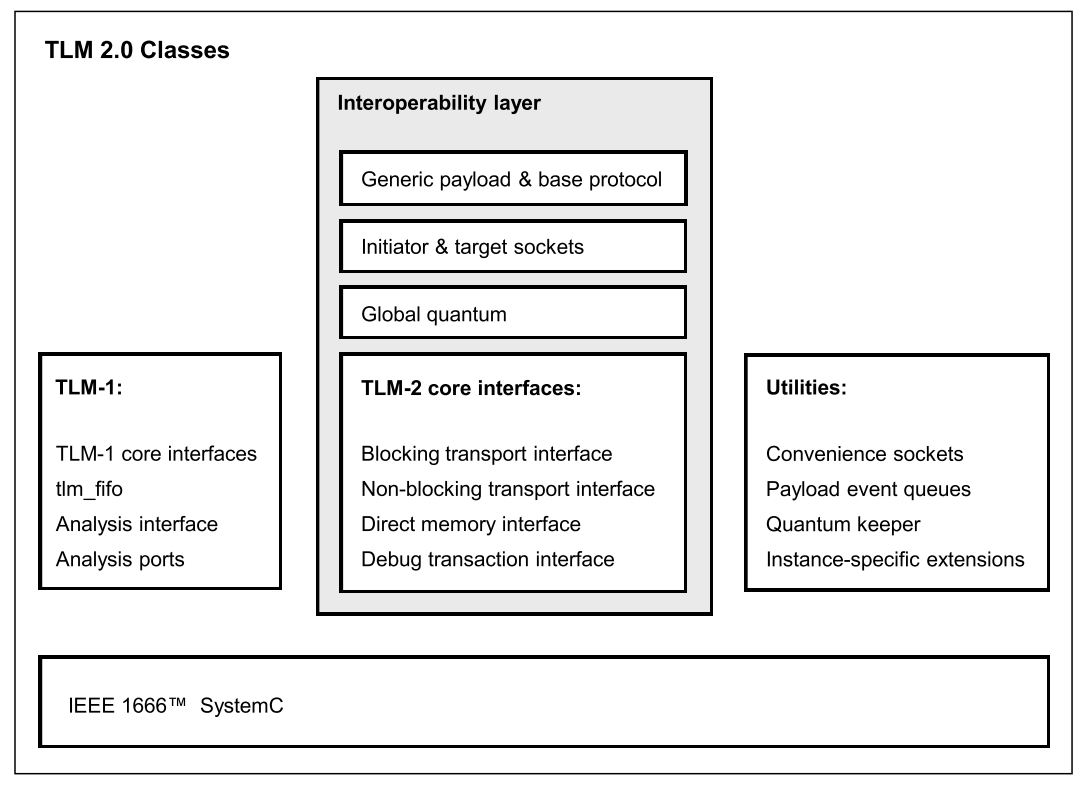
\includegraphics[scale=.3]{Figures/TLM_features.png}
\caption{\label{fig:TLM_features}TLM 2.0 use cases (adopted from \cite{OpenSystemCInitiative2009}).}
\end{figure}


\subsection{Transactions, Sockets, Initiators and Targets}
\label{sec-6-2}
\textbf{Transactions} are non-atomic communications, normally with bidirectional data transfer, and consist of a set of messages that are usually modeled as atomic communications.
In a transaction one can distinguish two roles;
the \textbf{initiator}, the component which initiated the communication, and the \textbf{target}, the component which is supposed to service the initiator's request.
A component is not limited to either of these two roles; it can assume both.
For example, \textbf{interconnect} components encapsulate the behavior of memory-mapped buses, being responsible for routing transactions to the correct target.
From the initiator's perspective, they act as targets and from the target's perspective they act as initiators.

Implementation-wise, communication in TLM 2.0 is reduced to method calls, 
from the initiator to the target through an arbitrary number of interconnect component, without involving any context switches from the simulation kernel.

A component's role is signified by the type of \textbf{sockets} it contains.
Initiator sockets are used to forward method calls "up and out of" a component, while target sockets are used to allow method calls "down and into" a component.
Socket binding is the act of connecting components together, thus defining the component whose method call will be eventually executed to service the transaction.
From SystemC's viewpoint, a socket is basically a convenience class, wrapping a \texttt{sc\_export} and a \texttt{sc\_port}.

\uline{COMMENT:} Maybe explain in more detail SystemC's export and port mechanisms?
Maybe you need to adopt a more SystemC like terminology? For example change the word "component" to "module".


\subsection{Generic Payload}
\label{sec-6-3}
The basic argument that is passed, by reference, in communicative method calls is called the \textbf{generic payload}.
It is a structure that contains all the necessary information about the transaction.
It supports the abstract modeling of memory-mapped buses, together with an extension mechanism to support the modeling of specific bus protocols whilst maximizing interoperability.

The main features/fields of the generic payload are:
\begin{itemize}
\item Command 
Is it read or write?
\item Address
What is the address, who is supposed to serve the transaction.
\item Data
A pointer to the physical data as an array of bytes.
\item Phase
Since a transaction is a non-atomic operation, this indicates the stage of the transaction. It is used for a detailed modeling of communication protocols.
\item Response
An enumeration, indicating whether the transaction was successful, and if not, what is the nature of the error.
\end{itemize}




\subsection{Coding Styles}
\label{sec-6-4}
LT is suited for describing virtual platforms intended for software development.
However, where additional timing accuracy is required, typically for software performance estimation and architectural analysis use cases, the AT style is employed.
Virtual platforms typically do not contain many cycle-accurate models of complex components because of the performance impact. 

\uline{COMMENT:} This is a quite problematic section. You need to elaborate more, do not forget LT is on your thesis title. 


\subsection{An Example}
\label{sec-6-5}
This unit will provide a literate code listing for the model in figure \ref{fig:TLM_tutorial}
\begin{figure}[htb]
\centering
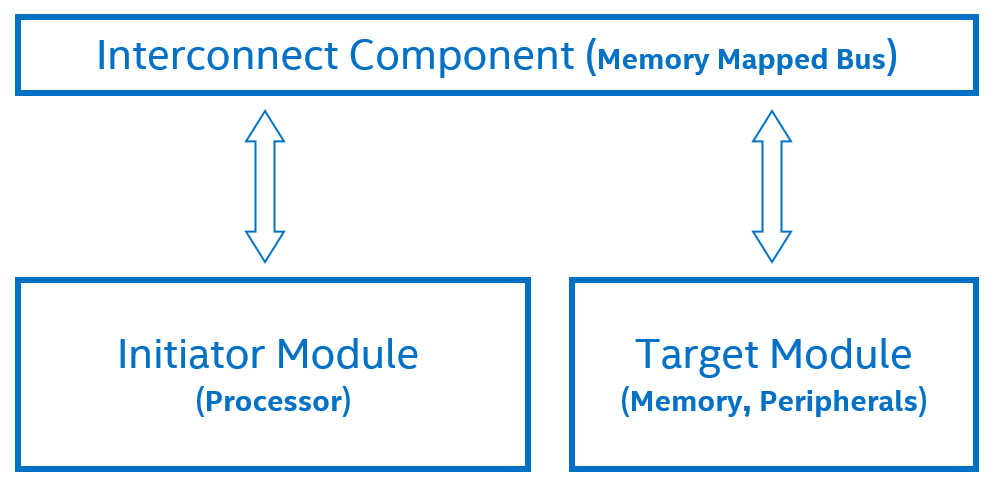
\includegraphics[scale=.4]{Figures/TLM_tutorial.png}
\caption{\label{fig:TLM_tutorial}A simple system-level model. The initiator, for example, could model a processor, the interconnect component a memory bus and the target a memory.}
\end{figure}


\subsection{Criticism}
\label{sec-6-6}
The root problem with TLM 2.0 lies in the elimination of explicit channels, which were a key contribution in the early days of research on system-level design.
As most researchers agreed, the concept of separation of concerns was of highest importance, 
and for system-level design in particular, this meant the clear separation of computation (in behaviors or modules) and communication (in channels).
Regrettably, SystemC TLM 2.0 chose to implement communication interfaces directly as sockets in modules and this indifference between channels and modules thus breaks the assumption of communication being safely encapsulated in channels.
Without such channels, there is very little opportunity for safe parallel execution \cite{Liu2015}.

For the above reason some designers consider TLM 2.0 a step towards the wrong direction and revert back to TLM 1.0.
Do you agree with this trend? 
Maybe tell us the major difference with TLM 1.0?

This is why SystemC TLM 2.0 model needs to be \textbf{recoded} to allow parallel execution.
The recoding must reconstitute the separation of concerns between computation and communication.
A modification of just the kernel will not suffice.



\subsection{Simics and TLM 2.0}
\label{sec-6-7}
Everything you do with SystemC TLM 2.0 you can do with Simics.
Simics is the main alternative to SystemC TLM 2.0 for system-level design.

\uline{COMMENT:} Can you briefly outline the differences between the two tools/frameworks?
Is Simics capable of PDES?
\clearpage


\section{Use Case}
\label{sec-7}
In this chapter we describe the transaction level model we are going to use for conducting our experimentation.
The purpose of the experimentation is twofold;
verify whether we achieve better faster simulation compared to the reference SystemC kernel and evaluate the proposed process synchronization algorithms.

\subsection{Platform modeling}
\label{sec-7-1}
A block diagram of the platform that will be modeled is seen in figure \ref{fig:Platform}.
The platform is a shared memory, cache-coherent, symmetric multiprocessor system based on the \href{http://opencores.org/or1k/Or1ksim}{OpenRisc 1200 Instruction Set Simulator}.
Cache coherence is enforced by a directory residing in the inclusive L2 cache.
Every component is/will be implemented in C/C++ and wrapped in SystemC modules using the TLM 2.0 API for communication. 
The exact number of processors is yet to be determined.

\begin{figure}[htb]
\centering
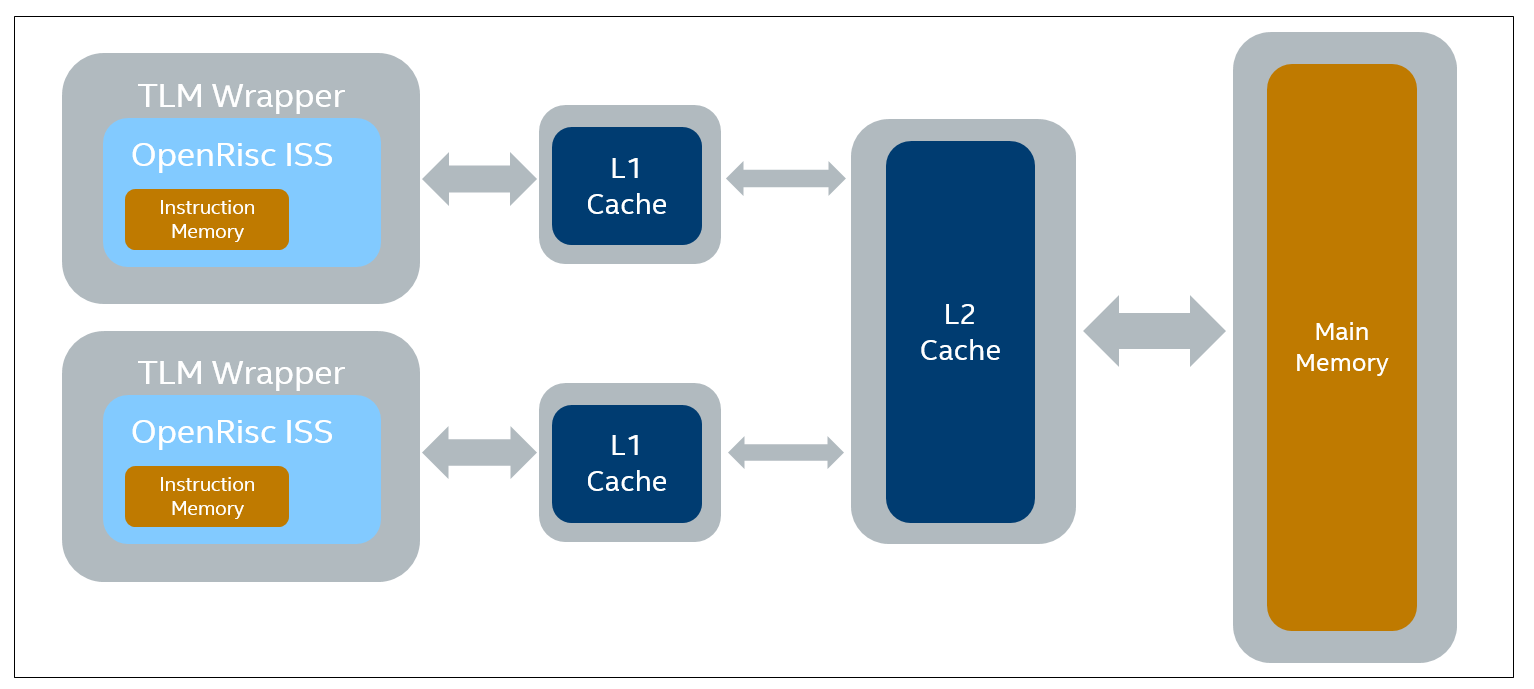
\includegraphics[width=.9\linewidth]{Figures/platform.png}
\caption{\label{fig:Platform}A model of a shared memory, cache-coherent, symmetric multiprocessor system}
\end{figure}


\uline{COMMENT:} Can you be more specific about the cache coherence protocol? Maybe provide a state diagram?


\subsection{Application modeling}
\label{sec-7-2}
We have the bare metal (newlib based) toolchain for compiling applications for the OpenRisc ISS.

\uline{COMMENT;} What kind of application am I going to run on this platform?
I see that most of the papers out there do some kind of mpeg2 decoding. That seems complex.

\clearpage




\section{References}
\label{sec-8}
\renewcommand\refname{}
\bibliography{References}
\bibliographystyle{myIEEEtran}
% Emacs 24.5.1 (Org mode 8.2.10)
\end{document}
